
\section{Styrenhet}

Styrenheten har till uppgift att driva de motorer som driver hjulen och de servon som styr armen.

\subsection{Övergripande struktur}

Styrenheten består av en AVR av typ Atmega16, två motorpar och en robotarm av typ Trossenrobotics Reactor. AVRen är ansluten till huvudenheten med en UART-buss och en \todo{två?} busy-pinne. Kommandon från huvudenheten fås enligt protokoll definierat i sektion \ref{protokoll:pc-motor}.\\

\todo{Schema över styrenheten}

\subsection{Framdrivning}

Styrenheten innehåller två motorpar. De är anslutna med två PWM-signaler till AVRen, en till höger respektive vänster hjulpar. Från huvudmodulen får styrenheten önskad hastighet på vardera hjulpar, vilka den applicerar och har så möjlighet att styra roboten framåt, bakåt, höger och vänster. Styrmodulen är ansvarig för att i mjukvara implementera acceleration av motorerna så att roboten rör sig mjukt genom sin omvärld.

\subsection{Robotarm}

Robotarmen består av 7 servon av modell AX12-A. De är anslutna med AVRen med en UART-buss. Dessa servon styrs genom att en målvinkel sätts (0-1023) med möjlighet att ändra hastighet, vridmoment och styra av/på. Från huvudmodulen får styrenheten målvinklar för varje enskild led. Styrmodulen är ansvarig för att se till att parallella servon körs synkroniserat för att inte slita sönder varandra. Styrmodulen är också ansvarig för att servona accelerar och bromsar något i sina rörelser för att robotarmen inte skall röra sig mjukt och utan ryck. Så länge robotarmen är i rörelse sätts en busy-flagga. Den låter huvudenheten utföra köade kommandon för robotarmen så snart som det är möjligt. 

\begin{figure}[h]
\center
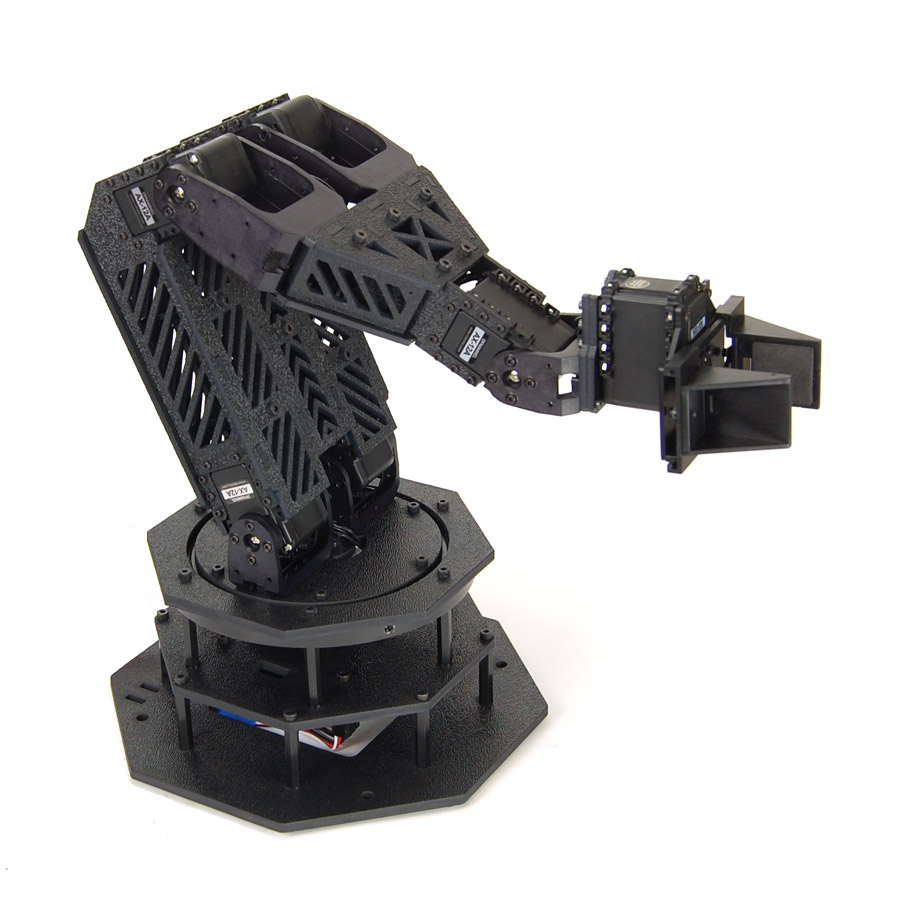
\includegraphics[scale=0.35]{arm}
\caption{Trossenrobotics Reactor.}
\end{figure}

\subsection{Mjukvara}

Mjukvaran på styrenhetens AVR kommer huvudsakligen skrivas i C. Eftersom kommunikation med huvudmodulen sker med UART, kommer mjukvaran huvudsakligen vara avbrottsdriven. Vid mottaget kommando via UART sker ett avbrott och enheten lagrar data eller utför tidigare givna kommandon. Den tid som spenderas utanför avbrottsrutinerna används för att accelerera och bromsa motorer och servon. AVRen hämtar status för alla servon, vilken position och hastighet de har och jämför dessa värden med målpositionerna. Efter analys av dessa data ges nya hastigheter till servon och motorer. \\
Vid de tillfällen AVRen kommunicerar med servona genom UART bör alla avbrott slås av.  \\

\todo{Flödesschema för AVR}